
%\documentclass[10pt, conference, compsoc]{IEEEtran}
\documentclass[times, 10pt,twocolumn]{article}

\usepackage{sose2011}
\usepackage{times}

%S\usepackage{fancyheadings}

%\ifCLASSINFOpdf
  \usepackage[pdftex]{graphicx}
  % declare the path(s) where your graphic files are
  \graphicspath{{./images/}}
  % and their extensions so you won't have to specify these with
  % every instance of \includegraphics
  \DeclareGraphicsExtensions{.pdf,.jpeg,.png,.jpg}
%\else
  % or other class option (dvipsone, dvipdf, if not using dvips). graphicx
  % will default to the driver specified in the system graphics.cfg if no
  % driver is specified.
%  \usepackage[dvips]{graphicx}
  % declare the path(s) where your graphic files are
%  \graphicspath{{./images/}}
  % and their extensions so you won't have to specify these with
  % every instance of \includegraphics
%  \DeclareGraphicsExtensions{.eps}
%\fi

% correct bad hyphenation here
\hyphenation{op-tical net-works semi-conduc-tor}

\begin{document}
%
% paper title
% can use linebreaks \\ within to get better formatting as desired
\title{Managed Control of Composite Cloud Systems}


% author names and affiliations
% use a multiple column layout for up to two different
% affiliations
%\author{\IEEEauthorblockN{Christopher C. Lamb, Pramod A. Jamkhedkar, Gregory L. Heileman}
%\IEEEauthorblockA{University of New Mexico\\
%Department of Electrical and Computer Engineering\\
%Albuquerque, NM 87131-0001 \\
%\{cclamb, pramod54, heileman\}@ece.unm.edu}
%}

\author{
        \textbf{Christopher Lamb}\hspace*{0.3in}
        \textbf{Pramod Jamkhedkar}\hspace*{0.3in}
        \textbf{Greg Heileman}\\
        Department of Electrical and Computer Engineering \\
        University of New Mexico \\
        \small{\{cclamb, pramod54, heileman\}@ece.unm.edu}
}

% make the title area
%\maketitle
\maketitle

\begin{abstract}
abstract
\end{abstract}

\textbf{Keywords:} Usage Managment, Cloud Computing, System of Systems.

%\begin{IEEEkeywords}
%usage management; personal medical records
%\end{IEEEkeywords}

%\IEEEpeerreviewmaketitle

\section{Introduction}
Cloud computing provides computing infrastructure and applications in the form of sophisticated services that can be accessed over a network. In cloud computing usage scenarios,  data and applications  of a ``cloud user'' reside on the cloud computing infrastructure that is owned and maintained by a third party ``cloud provider''.  This particular characteristic of cloud computing raises a number of policy issues in terms of user concerns and expectations, which include service reliability, liability, security, privacy, access control, usage control and protection of intellectual property~\cite{JeLiGr:08}.  Typically, these user expectations are captured in the form of Service Level Agreements (SLAs) that are brokered between the providers and users~\cite{BuYeVeBrBr:09}. The proposed research will explore the theoretical and practical aspects of developing a framework that will provide a comprehensive solution for expression, evaluation, reasoning and management of SLA policies in cloud computing environments in an automated manner. 

The proposed research plan will be carried out in three phases. The first phase will focus on studying the requirements for expression semantics to capture cloud computing SLAs, and subsequently  designing a formal language for policy expression that will accurately capture the desired semantics. The next phase will involve design and development of a framework for usage management in cloud computing environments, wherein the policy language for cloud computing will be incorporated. The framework will provide usage management services to other cloud computing services for expression, reasoning and validation of cloud policies on handling of data and applications. In the final phase of the research the framework will be deployed in existing cloud environments. This task will include a study of how the framework can leverage existing negotiation mechanisms, service and data aggregation techniques, encryption mechanisms, and  trusted computing technologies  to provide comprehensive cloud computing security solutions. 

\subsection{Previous Work}
prev

\section{New Models}
A cloud user, in a cloud computing scenario, has legitimate concerns with respect to security, privacy, access control, protection of intellectual property, etc., of the data, and these concerns are translated into legally binding service level agreements (SLAs) that are brokered between the cloud user and cloud provider. At present, such SLAs are generally represented in a natural language, and the security policies offered by the cloud providers are often rudimentary with one-size-fits-all options. For example, the Amazon S3 service for data storage allows users to choose a geographical region where their data would be stored, and guarantees that the data will never leave the selected region. Furthermore, in most cloud computing solutions, the interpretation of the SLAs, and their enforcement and monitoring within a cloud environment are carried out in a static manner as shown in Figure~\ref{fig:overview}.

\begin{figure}[!t]
\centering
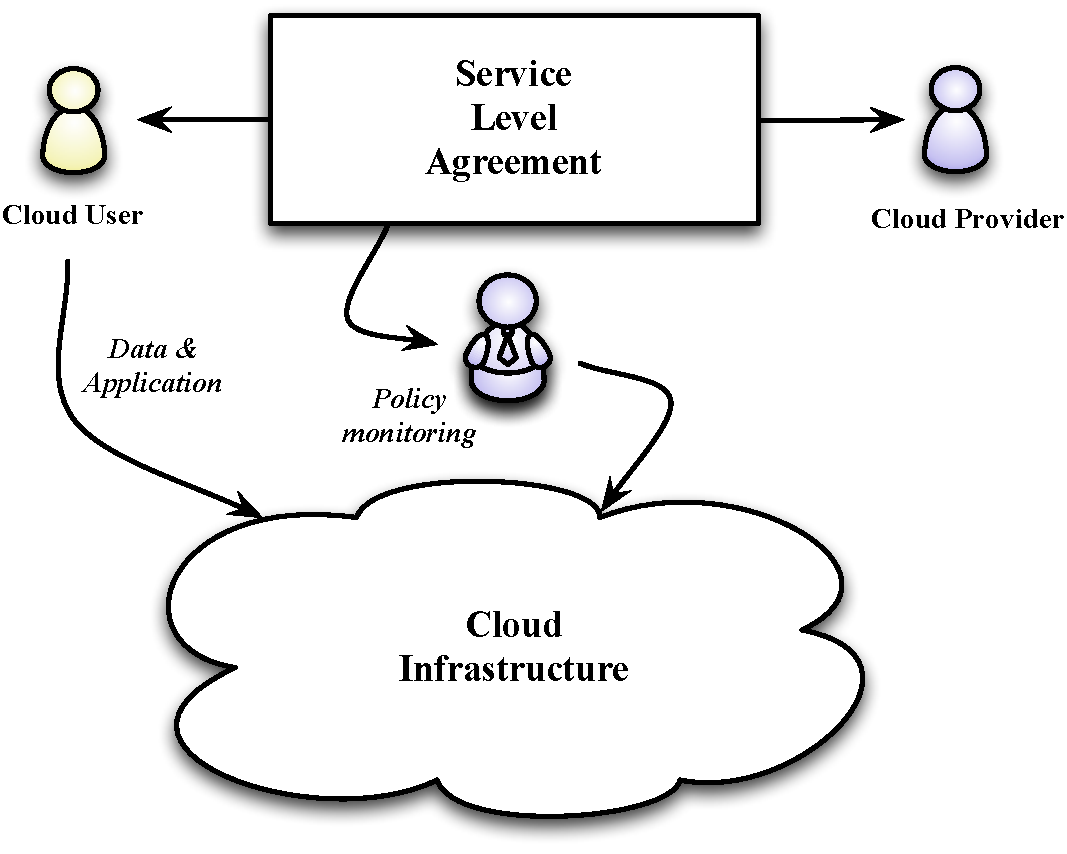
\includegraphics[width=3in]{Overview.pdf}
% where an .eps filename suffix will be assumed under latex, 
% and a .pdf suffix will be assumed for pdflatex; or what has been declared
% via \DeclareGraphicsExtensions.
\caption{Overview of the manner in which SLAs are implemented in present cloud environments.}
\label{fig:overview}
\end{figure}

The manner in which SLAs are presently expressed, interpreted, enforced and monitored has a number of shortcomings that will pose a serious impediment in creating secure cloud computing solutions of the future.  A  rudimentary policy option on data security leaves little room for cloud users to express and negotiate their security concerns and requirements. Ideally, an SLA must allow both parties to negotiate the service terms in an agreement that is expressive enough to capture the requirements and concerns of the parties involved. The cloud computing systems of the future will therefore require a user customized fine-grained SLAs as opposed to the current one-size-fits-all model. Another limitation of the present approach is that security policies expressed in SLAs are non-actionable, and their interpretation and enforcement is hardwired into the system. This approach makes it difficult to interpret an SLA with respect to the specifics of the underlying cloud computing infrastructure, and leverage the existing security features such as encryption mechanisms, trusted computing platforms, authentication mechanisms, etc., to enforce and monitor the SLA policies. 

In order develop secure cloud computing solutions of the future, it is necessary to have a mechanism in place that will allow a fine-grained expression of SLAs in a machine actionable format, and dynamically interpret, enforce, and monitor them while leveraging the specifics of the underlying cloud infrastructure. Such a mechanism will bring about radical changes to the manner in which SLAs are managed, and will open up numerous business opportunities to provide enriched cloud services. Actionable, machine-readable representation of fine-grained policies will open up the possibility of providing automated agent-based negotiation between cloud users and cloud providers. If policies are made actionable, it will enable the cloud providers to reason over the policy to manage and allocate its resources in an optimal manner. The ability to reason over a policy, and allocate and manage cloud resources with respect to a policy will allow cloud providers to estimate the cost associated with enforcing a policy, which in turn will enable price differentiation based on security policies requested by cloud users.
 
The proposed research plan includes the design and development of an open, interoperable framework that will allow automated expression, interpretation, enforcement, reasoning and monitoring of machine readable SLAs with respect to underlying cloud infrastructure. Figure~\ref{fig:cloud-umf} shows the manner in which the proposed framework will operate within cloud environments, as compared to the present approach which is shown in Figure~\ref{fig:overview}. As shown in Figure~\ref{fig:cloud-umf}, initially, the cloud provider and the cloud user negotiate the terms of SLA. The provisioning of machine readable and actionable SLAs that can be reasoned over will enable such negotiations to be carried out in an automated manner making use of existing negotiation protocols and agent development frameworks~\cite{BePoRi:02,FIPA}. The price associated with enforcing the negotiated SLA is then determined and conveyed to the cloud user. Once the terms are agreed upon, they are represented in a formal policy specification language that can be queried and reasoned over. The usage management framework will be deployed over a distributed cloud infrastructure to enable interpretation, and enforcement of the SLA in congruence of with security mechanisms available in the cloud infrastructure. The framework will provide an open platform with appropriate interfaces to plug-in different security mechanisms in conjunction with a policy reasoning module to construct comprehensive cloud security solutions. The development of such an open framework will be built upon the previous work of PIs involving the design of open framework for usage management, interoperability in rights management systems, and formal policy languages~\cite{JaHe:09,JaHeLa:10}.


\begin{figure}[!t]
\centering
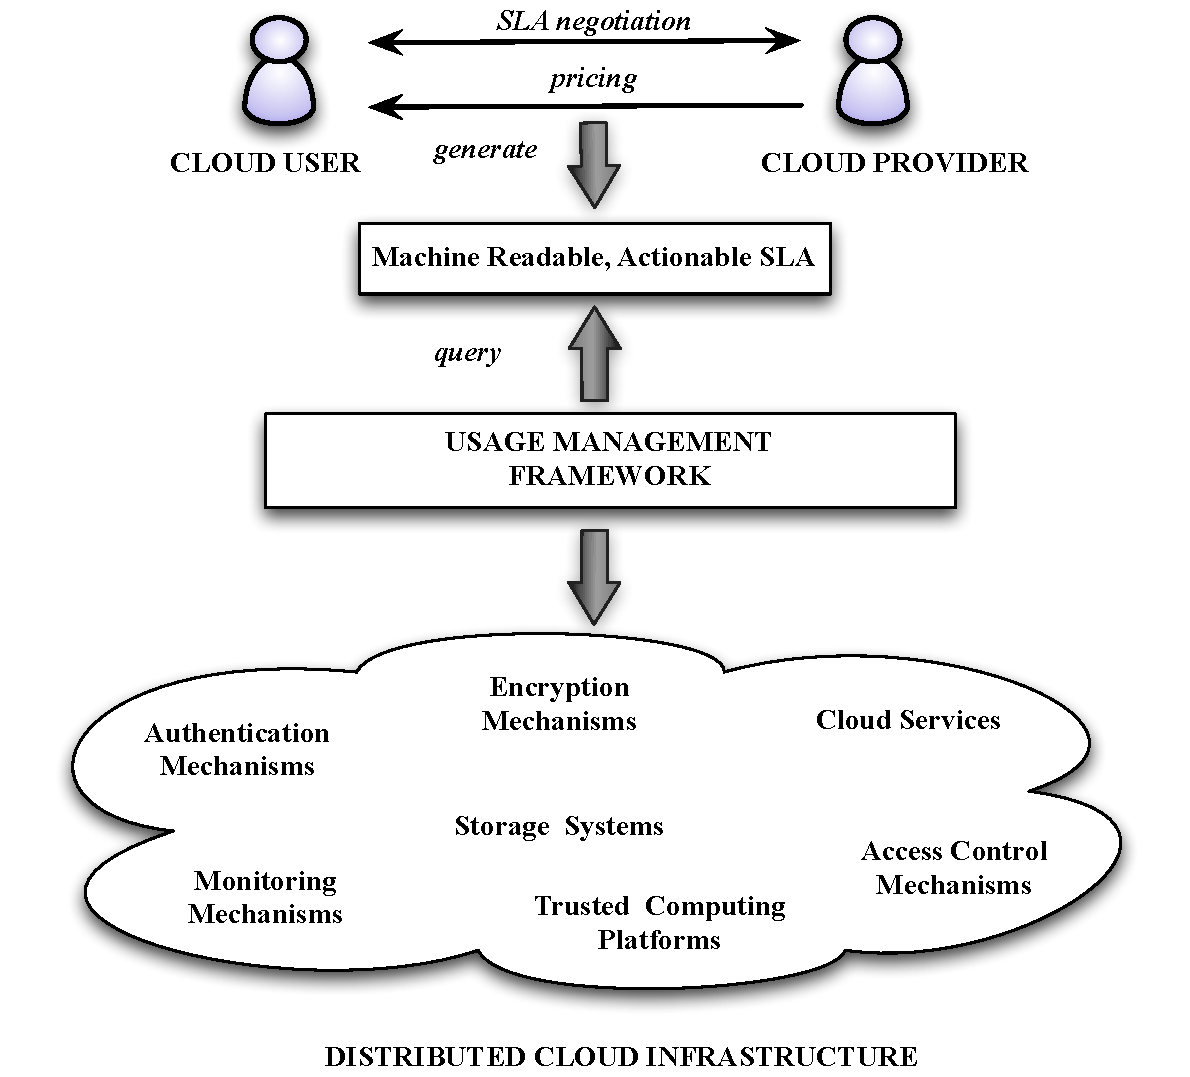
\includegraphics[width=3in]{cloud-umf.pdf}
% where an .eps filename suffix will be assumed under latex, 
% and a .pdf suffix will be assumed for pdflatex; or what has been declared
% via \DeclareGraphicsExtensions.
\caption{Usage management framework deployed in cloud environments}
\label{fig:cloud-umf}
\end{figure}

The development of such an open framework for SLAs involves a number of challenges and needs to exhibit certain features that are specific to cloud computing usage scenarios. A cloud computing environment is distributed and dynamic in nature, and cloud computing usage scenarios typically involve the employment of a number of cloud services possibly made available by different cloud providers. In order for the framework to provide a consistent policy reasoning mechanism, it is necessary that all the players, i.e. the cloud services and service providers agree on a common cloud ontology to ensure that the interpretation of SLAs is consistent across different cloud services. The first task of the research will involve the development of an a cloud computing ontology that will be used by different entities operating within the framework. The development of such an ontology will be carried out and represented in formal ontology modeling tools such as Protege. 

The second task in the research plan will involve development of a formal policy specification language that will be used within the framework for expressing and interpreting SLAs in an automated manner.  The dynamic and distributed nature of cloud computing implies that multiple cloud services, owned by different cloud providers, handle data and applications from different cloud users, in a manner where fragments of data move through different cloud services during the lifecycle of the application. The proposed policy language will handle scenarios where cloud services are able to reason over SLAs persistent through data transformation including fragmentation and aggregation. An example of such a usage scenario, involving data aggregation, is shown in Figure~\ref{fig:dynamics}. As shown in the figure, data from two different sources, each governed by its own SLA  policies is collected by the cloud service of  Service Provider 1. This cloud service aggregates the data from these two different sources, and generates a combined policy for the aggregated data. This aggregated data is then fed to a cloud service operated by Service Provider 2. In this example, the usage of the aggregated data is governed by the individual policies for the original data sets. In addition to that policies are generated via common cloud ontology to enable their consistent reasoning across different cloud providers. The proposed framework will be designed to handle such usage scenarios that reflect the dynamics of cloud environments. 

\begin{figure}[!t]
\centering
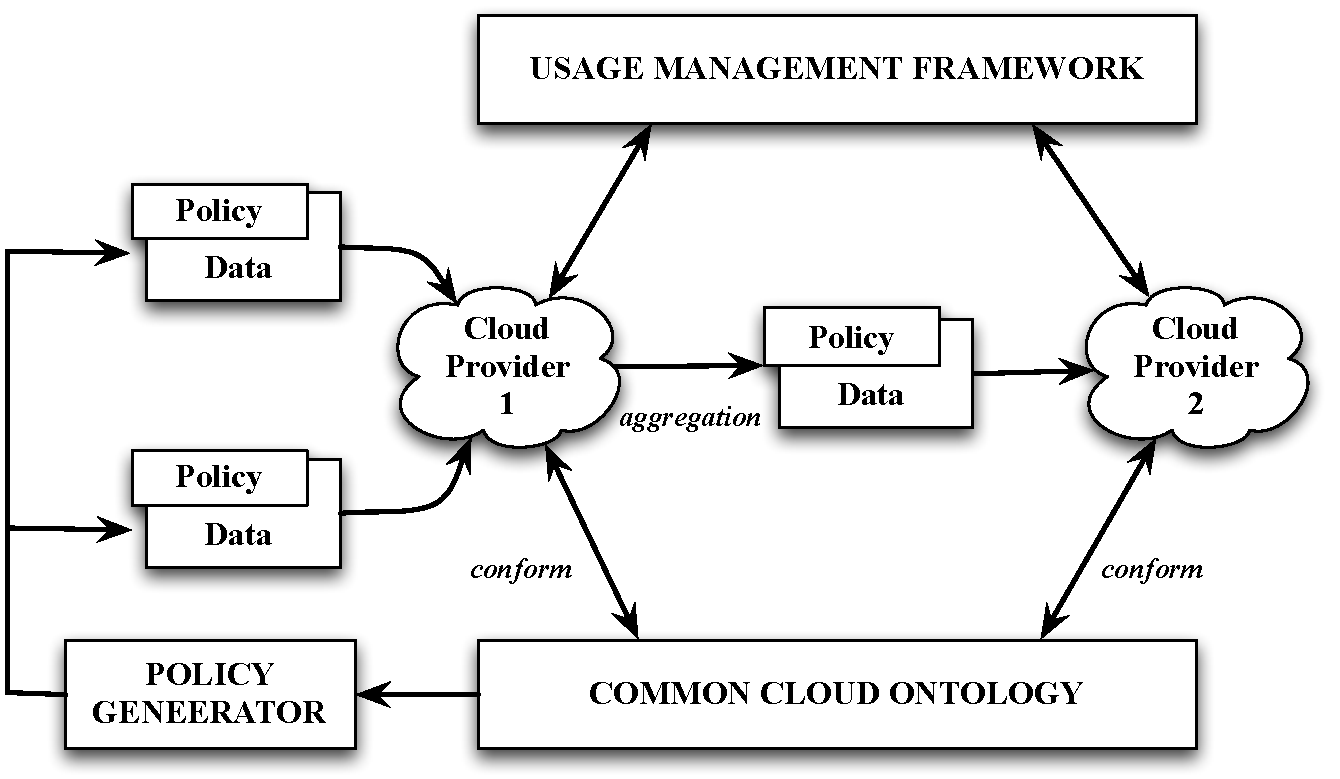
\includegraphics[width=3in]{dynamics.pdf}
% where an .eps filename suffix will be assumed under latex, 
% and a .pdf suffix will be assumed for pdflatex; or what has been declared
% via \DeclareGraphicsExtensions.
\caption{An example showing aggregation of data and policies, and use of a common cloud ontology across cloud providers to enable interoperability.}
\label{fig:dynamics}
\end{figure}

The third task in the development of the framework will involve design of interfaces to enable the operation of multiple security mechanisms within the framework. The design of such interfaces will involve identification of  focal points of interaction among the different components operating within a distributed cloud environment that will be the ideal candidates for standardization. Standardization is vital to enable sharing and collaboration among different cloud services~\cite{HPCloud1}. It via these standardized interfaces interactions among different security components will take place, including, querying a security policy, requesting a trusted computing platform to enforce access control or privacy, requesting for authorization, and other such security functions. These interfaces will be designed using modeling tools such as UML.


\section{System Architecture}
A highly expressive, fine-grained security policy leads to a number of challenges in terms of cloud design and implementation, and at the same time it  opens up numerous business opportunities to cloud providers. It is obligatory on the part of cloud provider to ensure that the policies negotiated in the SLA with cloud users are appropriately enforced in the cloud. Some of the challenges that arise due to complex security policies are listed below. 

\begin{enumerate}
\item To determine whether a given security policy can be enforced with the security infrastructure in place. To determine what aspects of a given policy can be enforced and what aspects cannot be enforced with the underlying security infrastructure. To understand the relationship between types of policy terms  and the infrastructure necessary to enforce it. 
\item The estimate the cost associated with enforcing a security policy.
\item To determine the optimal way to enforce a security policy for a given data set. How to allocate resources in an optimal manner while enforcing security policies for multiple data sets from different cloud users. 
\item To enforce a security policy in a distributed manner over multiple cloud services and cloud service providers.
\item To determine whether multiple security policies are compatible or non-compatible with each other.
\item To determine resultant security policies when handling multiple data sets from different cloud providers.
\end{enumerate}

\begin{figure}[!t]
\centering
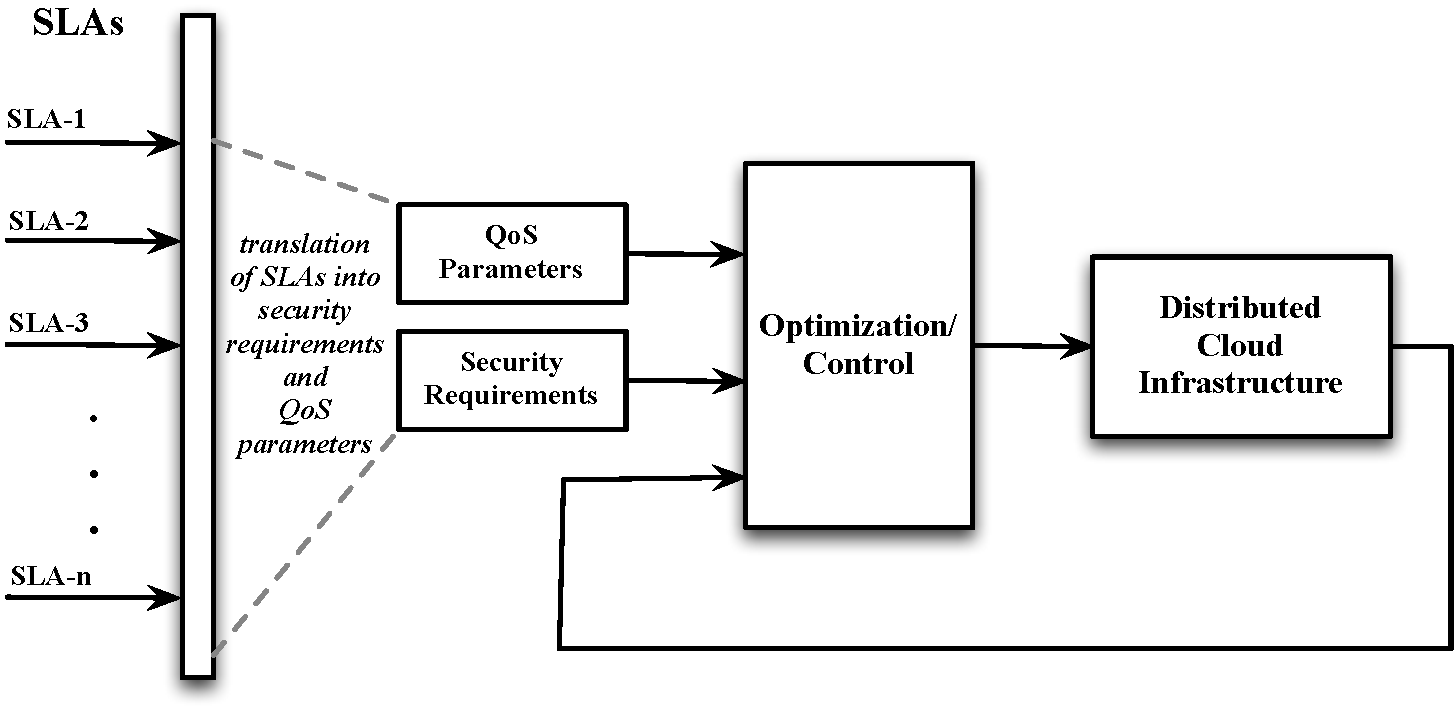
\includegraphics[width=3in]{cloud-security.pdf}
% where an .eps filename suffix will be assumed under latex, 
% and a .pdf suffix will be assumed for pdflatex; or what has been declared
% via \DeclareGraphicsExtensions.
\caption{Cloud control restricted by security policy}
\label{fig:cloud-security}
\end{figure}

It is necessary that these service level agreements are expressed in a formal machine readable language so that they can be interpreted and enforced in an automated manner in a cloud computing environment. There exists a rich body of previous work in the areas of access control, privacy and digital rights management that focusses on formal policy specification. However,  these solutions do not specifically take into account the challenges posed by the dynamics of cloud computing environments and usage scenarios. The proposed research will involve design and development of a formal framework to express, interpret and analyze the security requirements expressed in SLAs. 

The framework will address the challenges posed by the distributed and dynamic nature of cloud environments, and exploit the use of existing security mechanisms and trusted computing infrastructure solutions to be used within the framework to create secure cloud environments. The framework The particular challenges posed cloud environments in realization of this goal, and the manner in which they would be addressed in the research plan are described next.

Cloud computing environment is distributed in nature, and a cloud computing solution usually involves the use of multiple cloud computing services which are owned by different cloud providers. Each cloud service would employ a different SLA that may involve a different set of expression semantics. One of the key challenges in building the proposed framework is to identify and agree upon the type of semantics required in different cloud computing usage scenarios, and anticipate any semantics that might be required by future cloud computing systems. In order to address this challenge, instead of creating a standard policy expression language for SLAs, the proposed framework will provide a mechanism by means of which different languages can be used within the framework which can interoperate with different cloud computing services. Creating a standard policy specification language has three major flaws, namely, i)  in order to encompass all types of semantics such a language will become bloated, difficult to formalize and reason over, ii) such an approach will stifle innovation and  the language may be unable to incorporate any semantic needs that might arise in the future, and iii) it will take a lot of traction for all the players to agree on such a language as is evident in other areas such as digital rights management.

The proposed framework will provide a platform upon which different languages with varying degrees of expressive and reasoning power can be built and used within a distributed cloud environment by different cloud services.  To enable the use of multiple policy languages to interoperate in a common distributed cloud environment, it is necessary standardize certain aspects over which the languages agree upon and hide certain features of the language from the external world. The proposed research will involve identification of what characteristics of policy languages need to standardized and what characteristics need to be left free for innovation and differentiation. From their previous work, the PIs have demonstrated that in order to enable interoperability and use of multiple policy languages in a distributed environment there are two primary features that need to be standardized, namely, a common ontology and a policy query interface.

The proposed research will  involve the design of a common ontology for cloud computing environments that will be standardized and used across different cloud services. The development of such an ontology will be carried out and represented in formal ontology modeling tools such as Protege. This ontology will be extensible to incorporate requirements that might arise in the future, and will be shared by security components within distributed cloud environments to enable interoperability. In order design and develop this ontology, the research will involve a study of existing cloud solutions and a dialogue with standards bodies and cloud providers.

A standard, extensible interface for querying policy languages will be designed, that will be used by cloud services to query on the manner in which data needs to be handled. A web-bsed API for such an interface will be developed that will be adhered to by different policy languages. In prior research work, the PIs have successfully implemented and deployed a usage policy query API for multi-level security systems in DoD environment. The standard policy query interface will be a part of a larger research goal that will involve development of standard operational semantics for the framework, along with formal semantics to reason about interoperability among different entities within the framework. The focal points of interaction among the different components operating within a distributed cloud environment will be the ideal candidates for standardization. It via these standardized interfaces interactions among different security components will take place, including, querying a security policy, requesting a trusted computing platform to enforce access control or privacy, requesting for authorization, and other such security functions. These interfaces will be designed using modeling tools such as UML, and defined along the lines of other standards. 

The cloud environment is dynamic in nature in a number of ways. Multiple cloud services, owned by different cloud providers, handle data and applications from different cloud users, in a manner where fragments of data move through different cloud services during the lifecycle of the application. In addition to that, the properties of the cloud environment and that of the entities operating within the cloud are subject to frequent changes. The expression, interpretation, reasoning and enforcement of SLAs must take into account these dynamics of cloud environments.  In order to achieve this, the research will include development of a policy specification language that conforms to the framework standards, and takes into account these challenges. The language semantics will follow a clear separation between policy expression, interpretation and enforcement. The policy language will enable SLA policies to be expressed independent of cloud environment specifics, and allow the policy statements to be interpreted dynamically taking into account the specifics and the changes in the cloud environment within which the policy is being interpreted.  In order to manage the dynamic way in which data is handled, it is necessary that the policy persistent through data transformations occurring during the life time of the data. The proposed policy language will support selections, aggregations, transformations, etc., and reason policies over these data transformations. The policy language will enable cloud services to handle fractions of data from different sources in a manner that is consistent with the security policy of individual data sources. 

In addition to access control, a majority of the security concerns in SLAs reflect the manner in which data and applications are ``handled" or ``used" by the cloud.  Existing access control models or languages focus primarily on access restrictions, and therefore are incapable of expressing the usage aspects of the SLA policies. It is necessary that the policy specification model is able to handle a wide range of expression semantics including permissions, obligations, usage restrictions, privacy, rights protection, etc. One of the key challenges in this respect is to identify and agree upon the type of semantics that are currently used in cloud computing SLAs, and anticipate any semantics that might arise in future cloud computing systems. It is difficult to anticipate all the types of semantics that may be necessary for cloud applications. It is even more difficult to construct and reason over a formal specification language that will be able to capture all of these semantics. To address this problem, the proposed framework will include a policy specification model that will provide a scaffolding  upon which different types of specification languages can be built and used across different cloud computing services. Each such specification language can then be built using a type of mathematical logic that is best able to capture the necessary set of semantics. The characteristics that these policy specification model need to exhibit and the properties of the framework to enable the use of multiple specification languages along with other security mechanisms is described next. 

The proposed policy specification model upon which different languages will be built will provide a common cloud ontology that will be shared by by the policy specification languages.

In order to enable different specification languages to work within a common framework, the proposed framework will provide standard operational semantics and a common cloud ontology that will be shared across different entities within the framework. 

A cloud is a dynamic environment in which multiple cloud services, owned by multiple service providers, handle data and applications from multiple cloud users. In cloud environments, a single cloud service may handle fractions of data from multiple cloud users, and a set of data and applications of a single single cloud user may be divided into fractions and sent to different cloud services for handling. In such scenarios, it is necessary that each cloud service handles data fractions in such a way as to interpret and enforce the overarching security policy of the collective data set of the respective cloud user. 

The dynamics of the cloud environment is also reflected in the changes in the characteristics of the environment itself. A policy defined in the SLA needs to be independent of the changes in the cloud environment, which allows the policy to be defined on its own and interpreted appropriately depending on the current state or the type of the cloud environment. For example, an SLA might stipulate that the data is never routed though a hostile country. In this case the interpretation of the restriction ``hostile country" should be independent of a particular type of cloud environment, which may change as situations changes. 

In order to address these challenges, it is necessary that the policy model for expression, interpretation and enforcement of SLAs in cloud computing must be able to handle the dynamics of the cloud environment. In order for a formal framework to address these challenges, it must exhibit a certain set of features described below 

In order to handle a vast range of SLA policy semantics it is necessary that the policy model provides a framework in the form of a scaffolding upon which different types of formalisms can be built upon and used across different cloud computing services. In order to manage the dynamic way in which data is handled, it is necessary that the policy persistent through data transformations occurring during the life time of the data. The policy model must therefore support selections, aggregations, transformations, etc., and reason policies over these data transformations. In order to address the challenge of dynamics within the cloud environment and different types of cloud environments, the policy model must maintain a clear separation between policy expression, policy interpretation and policy enforcement. This will allow policies to be interpreted dynamically depending on type of the underlying cloud environment and be responsive to the changes that take place in that environment.  


%\begin{figure}[!t]
%\centering
%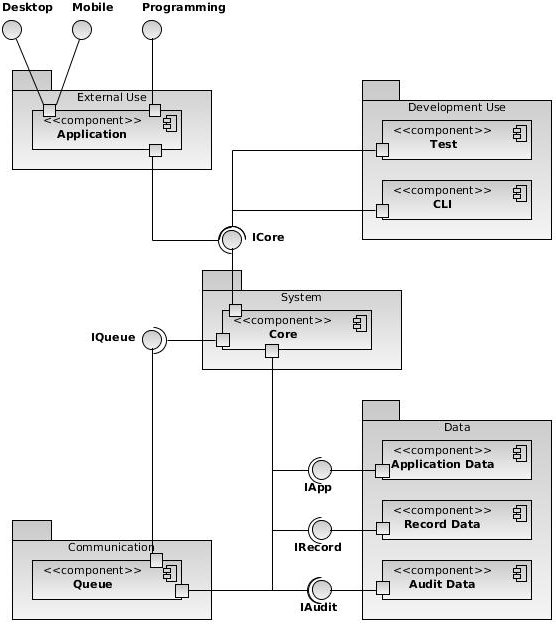
\includegraphics[width=3.4in]{HisbSystemArch}
%\caption{System Architecture Runtime Component View}
%\label{fig:RuntimeView}
%end{figure}

\cite{Emr:Web:Jade,Emr:Web:Fipa}.
\cite{KoLaMaMi:04,SaShUe:04}

\subsection{Sample System Architecture}
%Figure ~\ref{fig:RuntimeView} outlines a potential system architecture

\subsection{Usage Management}
 

\subsection{System Architecture and Attributes}

\section{Conclusion}

\bibliographystyle{IEEEtran}
\bibliography{emr,drm}

\end{document}


